\documentclass[11pt]{article}

\usepackage[english]{babel}         % American English
\usepackage[T1]{fontenc}            % Required for hyphenation
\usepackage[utf8]{inputenc}         % UTF-8 encoding

\usepackage{amssymb,amsmath,amsthm} % AMS
\allowdisplaybreaks                 % Math displays can break
\usepackage{url}                    % Typesetting URLs
\usepackage{hyphenat}               % Hyphenation with \hyp
\usepackage[scaled=0.8]{beramono}   % Nice bold/italic teletype font
\usepackage{float}                  % Tuning placement of figures
\usepackage{graphicx}               % Inclusion of graphics
\usepackage{caption,subfig}         % Subfigures
\usepackage{xspace}                 % Proper spacing after macros
\usepackage{alltt,calc}             % Verbatim with macros
\captionsetup[subfloat]{justification=raggedleft}
\usepackage[justification=raggedleft]{caption}
\usepackage{wrapfig}                % Wrapping text around figures
\usepackage[colorlinks=true,citecolor=black,linkcolor=black,urlcolor=blue]{hyperref}

\bibliographystyle{plain}  % TEMPORARY
%\usepackage{etoolbox}
%\apptocmd{\thebibliography}{\raggedright}{}{} % No Underfull \hbox

% New commands
%
\newcommand{\nb}[1]{\marginpar{{\color{red}\small #1}}}
\newcommand{\XML}{\textsf{XML}\xspace}
\newcommand\fig{\textsc{Figure}}
\newcommand\Fig{\textsc{Figure}}
%\renewcommand{\cdot}{\,}
\newcommand{\A}[2]{H_{#1}^{<#2}}
\newcommand{\B}[2]{H_{#1}^{\geqslant #2}}
\newcommand\Expected[1]{\mathbb{E}[{#1}]}

\title{The Average Height of Catalan Trees\\
  by Counting Lattice Paths}
\author{Nachum Dershowitz \and Christian Rinderknecht}
\date{}

\begin{document}

\maketitle

\hfill \emph{In memoriam} Philippe Flajolet, friend and colleague

\bigskip

Structured documents, like books, articles, and web pages, are composed
of chapters, sections, paragraphs, figures, appendices, indices, etc.
The
occurrences of these components are mutually constrained; for instance, it is
understood that a section is part of a chapter and that appendices are
located at the end of a document. This hierarchical layout is meant to
facilitate reading, and it supports the search for specific items of
information. When considering computer systems, these data must be
uniformly encoded by means of a formal language. 

Consider, for instance, an email message.
It contains at least the sender's address, a subject or title, the
recipient's address, and a body of text. These elements
correspond to \emph{nodes} arranged in a structure called a \emph{Catalan
  tree}, a.k.a.\@ an ordered tree or rooted plane tree. For example, the email
\begin{center}
\fbox{%
\begin{minipage}{\widthof{~~A \textbf{deadline} is a due date for a \emph{homework}.~~}}
\begin{alltt}
From: Me\\
Subject: Homework\\
To: You\\

A \textbf{deadline} is a due date for a \emph{homework}.
\end{alltt}
\end{minipage}
}
\end{center}
can be modeled by the tree in \fig~\ref{fig:mail},
\begin{figure}
\centering
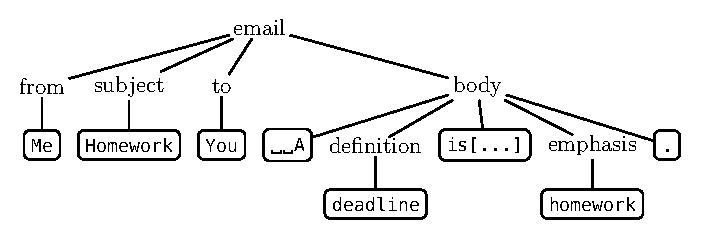
\includegraphics[bb=71 620 389 723]{mail}
\caption{An email viewed as a Catalan tree\label{fig:mail}}
\end{figure}
where the topmost node (``email'') is called the \emph{root} and the
framed pieces of text are \emph{leaves}.
Note that, for historical reasons, computer scientists grow
their trees upside down, with the root at the top. The inner (non-leaf) nodes hold ``metadata'', or ``markup'',
that is, information about the nature of the data contained in the subtree.

Catalan trees are a pervasive data structure in computer science, in
that they are a natural representation for hierarchical data. For
example, in \XML (eXtensible Markup Language), textual information is stored
in leaves, and, consequently, its retrieval requires
the traversal of the tree from the root to a leaf. The \emph{height}
of a tree is the number of nodes on a maximal path from 
root to leaf; for example, travel down the path with nodes depicted
as~\(\circ\) in the tree of height~\(5\) in \fig~\ref{fig:catalan}.
\begin{figure}
\centering
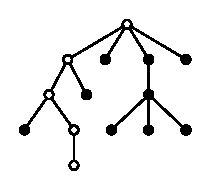
\includegraphics{catalan}
\caption{Catalan tree of height~\(5\) and size~\(13\).\label{fig:catalan}}
\end{figure}

In general, the maximum cost of a search is proportional to the height
of the tree, and the determination of the average height becomes
relevant when performing a series of random
searches~\cite{VitterFlajolet:1990}. The mathematical study of this
average quantity often relies on advanced analytical tools, and the
purpose of the present note is to propose a partial simplification of
these approaches by using elementary combinatorics.

\section*{The Analytical Derivation}

We measure the \emph{size} of a tree by the number of its edges; for
example, the tree in \fig~\ref{fig:catalan} is of size~\(13\).
Let~\(h_n\) be the average height of Catalan trees of size \(n\) and
\(H_{n}^{h}\) the number of Catalan trees of size \(n\) and
height~\(h\). We then have \(h_n = S_n/C_{n}\), where \(S_n := \sum_{h
  \geqslant 1} h \, H_{n}^{h}\), and~\(C_n := \binom{2n}{n}/(n+1)\) is
the number of Catalan trees of size \(n\).  The height of a tree with
$n$ edges can range from~$2$ (all leaves directly below the root) to
$n+1$ (one straight path from root to a lone leaf).

To gain purchase on the sum~\(S_n\), we may define~\(\A{n}{h}\) as
being the number of trees with \(n\)~edges and height less
than~\(h\). Then \(H_{n}^{h} = \A{n}{h+1}-\A{n}{h}\).  Of course, we
have \(\A{n}{h} = \A{n}{n+2} = C_{n}\), if \(h > n+1\).  Formulas can
be further simplified by letting~\(\B{n}{h}\) be the number of trees
with \(n\)~edges and height greater than or equal to~\(h\).  Now we
have:
\begin{equation}
S_n = \sum_{h \geqslant 1}h\left(\A{n}{h+1}-\A{n}{h}\right)
    = \sum_{h \geqslant 1}h\left(\B{n}{h}-\B{n}{h+1}\right) = \sum_{h\geqslant 1} \B{n}{h}.
\label{eq:Sn}
\end{equation} 
Knuth, de Bruijn, and Rice~\cite{KnuthdeBruijnRice:1972} published a
landmark paper in~\oldstylenums{1972}, where they obtained the
asymptotic approximation of the average height~\(h_n\). They started
by modeling the problem with a generating function~\cite{Wilf:1990}
that satisfies a recurrence equation whose solution expresses the
generating function in terms of continued fractions of Fibonacci
polynomials. Integration over complex numbers is then utilized to
obtain the formula
\begin{equation}
\B{n}{h} = \sum_{k \geqslant 1}\left[\binom{2n}{n+1-kh}
           - 2\binom{2n}{n-kh} + \binom{2n}{n-1-kh}\right].
\label{eq:Bn}
\end{equation}
The authors conclude by employing real and complex analysis to obtain
asymptotic expansions of~\(\B{n}{h}\), \(S_n\), and~\(h_n\). As we
will see, the main term is \(h_n \sim \sqrt{\pi n}\), where \(f(n)
\sim g(n)\) means \(\lim_{n \rightarrow \infty} f(n)/g(n) = 1\),
wherever \(f\)~and~\(g\) are defined.
  
The purpose of the present note is to show how to circumvent heavy
analytic techniques in the derivation of
equation~\eqref{eq:Bn}. Instead, we propose an elementary
combinatorial proof based on the enumeration of the Dyck paths of a
certain height, which are in bijection with Catalan trees of a related
height. We find this bijective proof to be more intuitive, in
particular to computer scientists, for whom the result matters for the
analysis of algorithms. Technically, our approach is in tune with
Mohanty~\cite{Mohanty:1979}, as well as Dershowitz and
Zaks~\cite{DershowitzZaks:1981}.

\section*{Counting Catalan trees}

Before we determine~\(\B{n}{h}\), let us solve a related and easier
question: deriving the number~\(C_n\) of Catalan trees with~\(n\)
edges, called the \emph{Catalan number}.

In \oldstylenums{1984}, Kemp~\cite[p.~64]{Kemp:1984} (see also
\cite{FlajoletNebelProdinger:2006}) derived equation~\eqref{eq:Bn} by
analytical means too, but, instead of working directly with Catalan
trees, he used certain lattice paths in an integer grid. 
\emph{Monotonic lattice paths}~\cite{Mohanty:1979,Humphreys:2010} are
made up of two kinds of steps, oriented upwards and oriented rightwards,
starting at \((0,0)\) with an upward step. \emph{Dyck paths} of
length~\(2n\) are monotonic paths ending at \((n,n)\) that never
venture below the diagonal; an example for \(n=6\) is shown in
\fig~\ref{fig:dyck}.
\begin{figure}
\centering
\subfloat[Dyck path of length 12.\label{fig:dyck}]{%
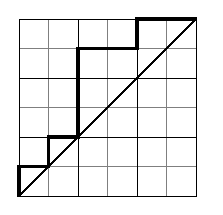
\includegraphics[bb=60 634 167 721]{dyck}
}
\qquad\qquad
\subfloat[Catalan tree with 6 edges.\label{fig:ctree}]{%
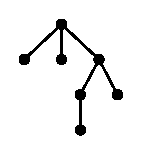
\includegraphics[bb=60 663 138 721,scale=1.5]{ctree}
}
\caption{Bijection between Dyck paths and Catalan trees.\label{fig:bijection}}
\end{figure}

\paragraph{A bijection with Dyck paths}

Crucially, there is a bijection between Dyck paths of length~\(2n\)
and Catalan trees with \(n\)~edges~\cite{Klarner}.

% Wrapping figure better declared before a paragraph
%
\begin{wrapfigure}[10]{r}[0pt]{0pt}
% 10 vertical lines
% right placement
% 0pt of margin overhang
\centering
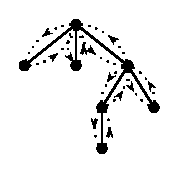
\includegraphics[scale=1.2]{preorder}
\caption{Preorder traversal \label{fig:preorder}}
\end{wrapfigure}
This bijection is shown on an example in \fig~\ref{fig:bijection}. To
construct the lattice path in \fig~\ref{fig:dyck} from the tree in
\fig~\ref{fig:ctree}, we imagine that the tree is a roadmap and our
avatar plans a tour starting at the root as follows: we take the
rightmost unvisited road (from the avatar's viewpoint), else we
backtrack: in the end, we have taken each road twice: there, and back
again. More technically, in \fig~\ref{fig:preorder}, we follow the
dotted arrows: each downward arrow in the tree corresponds to a step
up~\(\uparrow\) (called a \emph{rise}) in the lattice, and an upward
arrow in the tree to a step right~\(\rightarrow\) (called a
\emph{fall}). In the tree, the series is \(\downarrow\) \(\uparrow\)
\(\downarrow\) \(\uparrow\) \(\downarrow\) \(\downarrow\)
\(\downarrow\) \(\uparrow\) \(\uparrow\) \(\downarrow\) \(\uparrow\)
\(\uparrow\), which becomes \(\uparrow\) \(\rightarrow\) \(\uparrow\)
\(\rightarrow\) \(\uparrow\) \(\uparrow\) \(\uparrow\) \(\rightarrow\)
\(\rightarrow\) \(\uparrow\) \(\rightarrow\) \(\rightarrow\) in the
lattice. If we follow the latter from the start at the bottom left
corner \((0,0)\), we obtain the path in \fig~\ref{fig:dyck}. This kind
of traversal is called \emph{preorder}, or ``document'' order, because
it is the way we would read the document represented by the tree, from
cover to cover. Note as well that there are always~\(n+1\) nodes if,
and only if, there are~\(n\) edges in the tree, because there is
precisely one edge per node going up, save for the topmost node
(\emph{root}).

\paragraph{The inclusion-exclusion principle}

The previous bijection allows us to count the Catalan trees with
\(n\)~edges by counting instead the Dyck paths of length~\(2n\). 

It is easy to count all the monotonic paths of length~\(2n\) because
there are as many as choices of \(n\)~rises amongst \(2n\)~steps, that
is, \(\binom{2n}{n}\). To count only the Dyck paths, we need to
subtract the number of paths that start with a rise but cross below the
diagonal at some point.

This approach is a simple instance of the method known as the
\emph{inclusion\hyp{}exclusion principle}, whereby the direct and
difficult enumeration of a set is replaced by an easier enumeration
of a strict superset and the subtraction of the cardinality of a strict
subset, so that the resulting sets are equal.

% Wrapping figure better declared before a paragraph
%
\begin{wrapfigure}[14]{r}[0pt]{0pt}
% 14 vertical lines
% right placement
% 0pt of margin overhang
\centering
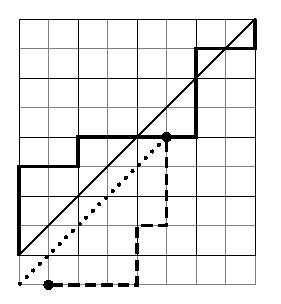
\includegraphics[scale=0.9]{reflection}
\caption{Reflection of a prefix with respect to \(y = x - 1\).
\label{fig:reflection}}
\end{wrapfigure}
An example of a path that is not a Dyck path is shown in
\fig~\ref{fig:reflection},
drawn in bold. The first point reached below the diagonal is used to
plot a dotted line parallel to the diagonal back to the $y$-axis. All
the steps on the path from that point back to \((0,0)\) are then
changed into their counterpart: a rise is replaced by a fall and
vice-versa. The resulting segment is drawn as connected dashed
lines. This operation is called a
\emph{reflection}~\cite{Renault:2008}. The crux of the matter is that
we can reflect each monotonic path crossing the diagonal into a
distinct path from \((1,-1)\) to \((n,n)\). These reflected paths can,
in turn, be reflected back into their original counterpart when they
reach the dotted line. In other words, the mapping is
bijective. (Another intuitive and visual approach to the same result
has been published by Callan~\cite{Callan:1995}.)  Consequently, there
are as many monotonic paths from \((0,0)\) to \((n,n)\) that cross the
diagonal as there are monotonic paths from \((1,-1)\) to
\((n,n)\). The latter are readily enumerated: \(\binom{2n}{n-1}\). In
conclusion, the number of Dyck paths of length~\(2n\) is
\begin{align}
C_n &= \binom{2n}{n} - \binom{2n}{n-1}
= \binom{2n}{n} - \frac{(2n)!}{(n-1)!(n+1)!}\label{eq:C}\\
&= \binom{2n}{n} - \frac{n}{n+1} \, \frac{(2n)!}{n!n!}
 = \binom{2n}{n} - \frac{n}{n+1} \binom{2n}{n} = \frac{1}{n+1}\binom{2n}{n}.\nonumber
\end{align}
Using Stirling's formula for the asymptotic equivalence, we draw the conclusion:
\begin{equation}
C_n = \frac{1}{n+1}\binom{2n}{n} \sim \frac{4^n}{n\sqrt{\pi n}},
      \quad\text{as \(n \rightarrow \infty\)}.
\label{eq:Cn}
\end{equation}

\section*{A Combinatorial Proof}

In~\oldstylenums{1996}, Sedgewick and
Flajolet~\cite{SedgewickFlajolet:1996,FlajoletSedgewick:2009} derived
the enumerations of Catalan trees by height, also using analytic
combinatorics, but they employed real analysis to obtain the
asymptotic approximation of~\(\B{n}{h}\). They
write~\cite[p.~260]{SedgewickFlajolet:1996}:
\begin{quote}
\it This analysis is the hardest nut that we are cracking in this
book. It combines techniques for solving linear recurrences and
continued fractions, generating function expansions, especially by the
Lagrange inversion theorem, and binomial approximations and
Euler\--Maclaurin summations.
\end{quote}

To avoid the aforementioned advanced techniques used to derive
equation~\eqref{eq:Bn}, we use again a bijection between Dyck paths
and Catalan trees, but, this time, the key point is that Catalan trees
of size \(n\) and height~\(h\) are in bijection with Dyck paths of
length~\(2n\) and height \(h-1\). This simple observation allows us to
reason about the height of the Dyck paths and transfer our findings
back to Catalan trees.

With the determination of~\(\A{n}{h}\) in mind, let us consider a Dyck
path of length \(2n\) and height~\(h-1\), as in \fig~\ref{fig:height}.
\begin{figure}
\centering
\subfloat[Dyck path of length \(2n\) and
height \(h-1\).\label{fig:height}]{
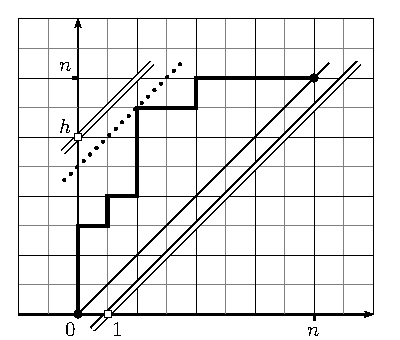
\includegraphics[bb=66 565 252 724,scale=0.9]{height}}
\qquad
\subfloat[Path from \(A\) to \(\Omega\) avoiding the boundaries
  \(y=x+s\) and \(y=x-t\).\label{fig:mohanty}]{
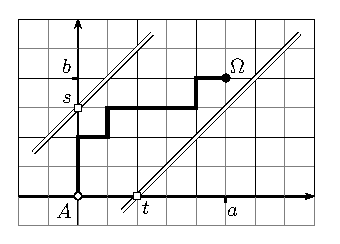
\includegraphics[scale=0.9]{mohanty}}
\caption{Paths avoiding diagonal boundaries.\label{fig:boundaries}}
\end{figure}
The double lines are boundaries that may not be attained by the
path. This is in fact a special case of a general monotonic path
between two diagonal boundaries, as shown in \fig~\ref{fig:mohanty},
where \(s\)~denotes the vertical distance from~\(A\), and \(t\),~the
horizontal distance from~\(A\). It is well known that the number of
monotonic paths from~\(A(0,0)\) to~\(\Omega(a,b)\) avoiding the
boundaries \(y = x + s\) and \(y = x - t\) is
\begin{equation}
\left\lvert\mathcal{L}(a,b;t,s)\right\rvert = \sum_{k \in \mathbb{Z}}\left[\binom{a+b}{b+k(s+t)} - \binom{a+b}{b+k(s+t)+t}\right].
\label{eq:mohanty}
\end{equation}
The proof by Mohanty~\cite[p.~6]{Mohanty:1979} of this formula is
based on the reflection principle and the principle of inclusion and
exclusion, which we used earlier. We quote his proof here verbatim,
because it is rarely found in print nowadays.
\begin{proof}[Proof {\rm (Mohanty~\cite{Mohanty:1979})}]
 For brevity, call the boundaries \(x=y+t\) and
  \(x=y-s\), \(\mathcal{L}^{+}\) and \(\mathcal{L}^{-}\),
  respectively. Denote by~\(A_1\) the set of paths that reach
  \(\mathcal{L}^{+}\), by~\(A_2\) the set of paths that reach
  \(\mathcal{L}^{+}\), \(\mathcal{L}^{-}\) in that order, and in
  general by~\(A_i\) the set of paths reaching \(\mathcal{L}^{+}\),
  \(\mathcal{L}^{-}\), \(\mathcal{L}^{+}\), \ldots\@ (\(i\)~times) in
  the specified order. Similarly, let~\(B_i\) be the set of paths
  reaching \(\mathcal{L}^{-}\), \(\mathcal{L}^{+}\),
  \(\mathcal{L}^{-}\), \ldots\@ (\(i\)~times) in the specified order. An
  application of the usual inclusion-exclusion method yields
\begin{equation}
\left\lvert\mathcal{L}(a,b;t,s)\right\rvert = \binom{a+b}{b} + \sum_{i
\geqslant 1}(-1)^{i}\left(\lvert{A_i}\rvert + \lvert{B_i}\rvert\right),
\label{eq:L}
\end{equation}
where~\(\lvert{A_i}\rvert\) and~\(\lvert{B_i}\rvert\) are evaluated by
using the reflection principle repeatedly. For example,
consider~\(A_3\). Since every path in~\(A_3\) must
reach~\(\mathcal{L}^{+}\), \(A_3\) when reflected about
\(\mathcal{L}^{+}\) becomes the set of paths from \((t,-t)\) to
\((a,b)\) each of which reaches~\(\mathcal{L}^{+}\) after reaching
\(\mathcal{L}^{-}\). Another reflection about \(\mathcal{L}^{-}\)
would make~\(A_3\) equivalent to the set of paths from \((-s-t,s+t)\)
to \((a,b)\) that reach~\(\mathcal{L}^{+}\), which in turn can be
written as \(R(a+s+t,b-s-t; 2s+3t)\). [Note: \(R(a,b;t)\) is the set
  of paths from \((0,0)\) to \((a,b)\) reflected
  about~\(\mathcal{L}^{+}\).] Thus, since \(\lvert{R(a,b;t)}\rvert =
\binom{a+b}{a-t}\), we have
\begin{equation*}
\left\lvert{A_3}\right\rvert = \binom{a+b}{a-s-2t},
\end{equation*}
and, more generally,
\begin{equation*}
\left\lvert{A_{2j}}\right\rvert = \binom{a+b}{a+j(s+t)}
\quad\text{and}\quad
\left\lvert{A_{2j+1}}\right\rvert = \binom{a+b}{a-j(s+t)-t}.
\end{equation*}
The expressions for \(\lvert{B_{2j}}\rvert\),
\(\lvert{B_{2j+1}}\rvert\), \(j=0, 1, 2, \dots\), with
\(\lvert{A_0}\rvert\), \(\lvert{B_0}\rvert\) being \(\binom{a+b}{b}\),
are obtained by interchanging \(a\)~with~\(b\) and
\(s\)~with~\(t\). Substitution of these values in~\eqref{eq:L}
yields~\eqref{eq:mohanty} after some simplifications.
\end{proof}

Resuming our argument, if we match the subfigures in
\fig~\ref{fig:boundaries}, we find \(s=h\), \(t=1\), \(a=b=n\),
hence \(a+b=2n\) and \(b+k(s+t)=n+k(h+1)\),
which we plug into formula~\eqref{eq:mohanty} and change \(h\)~into \(h-1\):
\begin{equation*}
\A{n}{h} = \sum_{k \in \mathbb{Z}}\left[\binom{2n}{n+kh} -
           \binom{2n}{n+1+kh}\right].
\end{equation*}
After splitting the sum into \(k<0\), \(k=0\), and \(k>0\), then
changing the sign of~\(k\) in the first case, using \(\binom{p}{q} =
\binom{p}{p-q}\) in the second, and lastly gathering the remaining
sums ranging over \(k \geqslant 1\), we reach
\begin{align*}
\A{n}{h}
  &= - \sum_{k \geqslant 1}\left[\binom{2n}{n+1-kh} -
    2\binom{2n}{n-kh} + \binom{2n}{n-1-kh}\right]\\
  &\phantom{=}\; + \binom{2n}{n} - \binom{2n}{n-1}.
\end{align*}
Recognizing \(C_n\) from equation~\eqref{eq:C}, we simplify as follows:
\begin{equation*}
C_n - \A{n}{h}
  = \sum_{k \geqslant 1}\left[\binom{2n}{n+1-kh} -
    2\binom{2n}{n-kh} + \binom{2n}{n-1-kh}\right].
\end{equation*}
Finally, recalling that \(\B{n}{h} =  C_n - \A{n}{h}\),
we arrive at
\begin{equation*}
\B{n}{h} = \sum_{k \geqslant 1}
            \left[\binom{2n}{n+1-kh} - 2\binom{2n}{n-kh}
            + \binom{2n}{n-1-kh}\right],
\end{equation*}
which is none other than our target, equation~\eqref{eq:Bn}.

In this way, we have achieved our goal merely by enumerating lattice
paths, and hopefully have, in the process, made this classic result
less daunting.

\section*{Asymptotics}

We could stop here, but we would like to give a hint as to how the
asymptotic approximation is carried out.  The approximation will give
us a practical handle on the expected height of Catalan trees, which
in turn tells us what to expect by way of performance of algorithms,
like search, that traverse down paths in arbitrary trees.

Equation~\eqref{eq:Sn}
entails \(S_{n} = \sum_{h \geqslant 1}\B{n}{h}\); therefore
\begin{equation*}
S_{n} = \sum_{k' \geqslant 1}d(k') %\cdot
        \left[\binom{2n}{n+1-k'} - 2\binom{2n}{n-k'}
        + \binom{2n}{n-1-k'}\right],
\end{equation*}
where~\(d(k')\) is the number of positive divisors of~\(k'\), but
complex analysis is
needed~\cite{KnuthdeBruijnRice:1972,FlajoletGourdonDumas:1995}. Another
way is to express the binomials in terms of \(\binom{2n}{n-kh}\):
\begin{align*}
\binom{2n}{n-m+1} &= \frac{(2n)!}{(n-m+1)!\,(n+m-1)!}\\
                  &= \frac{(2n)!\,(n+m)}{(n-m)!\,(n-m+1)(n+m)!} 
                   = \frac{n+m}{n-m+1}\binom{2n}{n-m},\\
\binom{2n}{n-m-1} &= \frac{(2n)!}{(n-m-1)!\,(n+m+1)!}\\
                  &= \frac{(2n)!\,(n-m)}{(n-m)!\,(n+m)!\,(n+m+1)}
                   = \frac{n-m}{n+m+1}\binom{2n}{n-m}.
\end{align*}
Therefore,
\begin{equation*}
\binom{2n}{n-m+1} - 2\binom{2n}{n-m} + \binom{2n}{n-m-1}
= 2 \, \frac{2m^2-(n+1)}{(n+1)^2-m^2}\binom{2n}{n-m}.
\end{equation*}
Let \(F_n(m) = (2m^2-n)/(n^2-m^2)\). We have
\begin{equation*}
S_{n} = 2 \, \sum_{h \geqslant 1}\sum_{k \geqslant 1} F_{n+1}(kh)
\, \binom{2n}{n-kh}.
\end{equation*}
From equation~\eqref{eq:Cn} and \(h_n = S_n/C_n\), we deduce \(h_{n} =
(n+1)S_{n}/{\binom{2n}{n}}\), hence we must approximate
\((n+1)F_{n+1}(m)\) and \(\binom{2n}{n-m}/\binom{2n}{n}\). On the
one hand, we have
\begin{equation*}
F_{n+1}(m) \sim \frac{2m^2-n}{n^2} \sim \frac{2m^2-n}{n(n+1)},
\end{equation*}
so \((n+1)F_{n+1}(kh) \sim 2k^2h^2\!/n-1\). On the other hand,
Sedgewick and Flajolet~\cite[4.6, 4.8]{SedgewickFlajolet:1996} show
\begin{equation*}
\binom{2n}{n-m}\bigg/{\binom{2n}{n}} \sim e^{-m^2\!/n}.
\end{equation*}
Assuming that the tails (the implicit error terms) of the two previous
approximations decrease exponentially, we have
\begin{equation*}
h_{n} \sim \sum_{h \geqslant 1}\sum_{k \geqslant 1}
(4k^2h^2\!/n - 2)e^{-k^2h^2\!/n}
= \sum_{h \geqslant 1}H(h/\!\sqrt{n}), 
\end{equation*}
where \(H(x) = \sum_{k \geqslant 1}(4k^2x^2-2)e^{-k^2x^2}\). Finally,
Sedgewick and Flajolet~\cite[\S 5.9]{SedgewickFlajolet:1996}, on the one
hand, and Graham, Knuth, and
Patashnik~\cite[\S 9.6]{GrahamKnuthPatashnik:1994}, on the other hand,
use real analysis to conclude
\begin{equation*}
h_n \sim \sum_{h \geqslant 1}H(h/\!\sqrt{n})
    \sim \sqrt{n} \int_0^{\infty}H(x) dx \sim \sqrt{\pi n}.
\end{equation*}
The end of this derivation is difficult because the error terms in the
bivariate asymptotic approximations must be carefully checked, so it
is unlikely to be simplified further. 

Remarkably, the main term $\sqrt{\pi n}$ in the asymptotic value for
the average height can also be obtained by simple lattice\hyp{}path
arguments~\cite{DershowitzZaks:1990}, as shown in the online
supplement to this article~\cite{Supplement:2015}.

\bibliography{lattice}
%%-*-latex-*-

\begin{abstract}
Recursion is a powerful programming technique which is notoriously
difficult to master, especially in functional languages because they
prominently feature structural recursion as the main control\hyp{}flow
mechanism. We propose several hypotheses to understand the issue and
put some to the test by designing an open\hyp{}source interactive
interface based on a tangible block\hyp{}world with augmented reality
and software feedback. Stacks of blocks are used as an analogy for the
list data structure, which enables the simplest form of structural
recursion. After using this application, students are expected to
transfer their training to directly write recursive programs in
sequential \erlang, a purely functional language.
\end{abstract}


\end{document}
